%%%%%%%%%%%%%%%%%%%%%%%%%%%%%%%%%%%%%%%%%%%%%%%%%%%%%%%%%%%%%%%%%%%%%%%%%%%%%%%%
%2345678901234567890123456789012345678901234567890123456789012345678901234567890
%        1         2         3         4         5         6         7         8

\documentclass[letterpaper, 10 pt, conference]{ieeeconf}  % Comment this line out
                                                          % if you need a4paper
%\documentclass[a4paper, 10pt, conference]{ieeeconf}      % Use this line for a4
                                                          % paper

\IEEEoverridecommandlockouts                              % This command is only
                                                          % needed if you want to
                                                          % use the \thanks command
\overrideIEEEmargins
% See the \addtolength command later in the file to balance the column lengths
% on the last page of the document


\usepackage{hyperref}

\usepackage{caption}
\usepackage{subcaption}
\usepackage{graphicx} % for pdf, bitmapped graphics files

% The following packages can be found on http:\\www.ctan.org
%\usepackage{graphics} % for pdf, bitmapped graphics files
%\usepackage{epsfig} % for postscript graphics files
%\usepackage{mathptmx} % assumes new font selection scheme installed
%\usepackage{times} % assumes new font selection scheme installed
\usepackage{amsmath} % assumes amsmath package installed
\usepackage{amssymb}  % assumes amsmath package installed

\title{\LARGE \bf
Tabletop Object Scanning with an RGB-D Sensor*
}

%\author{ \parbox{3 in}{\centering Huibert Kwakernaak*
%         \thanks{*Use the $\backslash$thanks command to put information here}\\
%         Faculty of Electrical Engineering, Mathematics and Computer Science\\
%         University of Twente\\
%         7500 AE Enschede, The Netherlands\\
%         {\tt\small h.kwakernaak@autsubmit.com}}
%         \hspace*{ 0.5 in}
%         \parbox{3 in}{ \centering Pradeep Misra**
%         \thanks{**The footnote marks may be inserted manually}\\
%        Department of Electrical Engineering \\
%         Wright State University\\
%         Dayton, OH 45435, USA\\
%         {\tt\small pmisra@cs.wright.edu}}
%}

\author{Maria Dimashova$^{1}$, Ilya Lysenkov$^{1}$, Vincent Rabaud$^{2}$ and Victor Eruhimov$^{1}$
\thanks{*This work was supported by Willow Garage, Inc.}% <-this % stops a space
\thanks{$^{1}$M. Dimashova, I. Lysenkov and V. Eruhimov are with Itseez, Nizhny Novgorod, Russia
        {\tt\small \{maria.dimashova, ilya.lysenkov, victor.eruhimov\}@itseez.com}}%
\thanks{$^{2}$V. Rabaud is with Aldebaran Robotics, Paris, France but part of this work was done while the author was 
at Willow Garage, Menlo Park, California, USA {\tt\small vrabaud@aldebaran-robotics.com}}%
}


\begin{document}



\maketitle
\thispagestyle{empty}
\pagestyle{empty}


%%%%%%%%%%%%%%%%%%%%%%%%%%%%%%%%%%%%%%%%%%%%%%%%%%%%%%%%%%%%%%%%%%%%%%%%%%%%%%%%
\begin{abstract}
This paper presents a complete pipeline for tabletop object scanning
which creates accurate 3D models from RGB-D data and can be carried out both by a person
and a robot. We consider the capturing scenario where a camera makes
a single turn around an object located on a table. The online part of our approach consists 
of initial camera motion estimation using RGB-D visual
odometry and detection of loop closure in the trajectory. The offline part
is graph-based global coarse-to-fine refinement of camera poses and model points.
In addition to the usual geometric ICP constraints, we add
RGB ones to make the scanning pipeline more stable in case 
of planar and symmetric surfaces. 
% With "in our specific case" it seems like we scan only planar and symmetric surfaces.

The presented object reconstruction pipeline was tested using both a hand-held RGB-D sensor and a PR2 robot.
As a result the algorithm successfully produced accurate models on a dataset of 42 household objects.
The code of our system is available as open-source.

%\TODO Make experiments with evaluation on ground truth models
\end{abstract}


%%%%%%%%%%%%%%%%%%%%%%%%%%%%%%%%%%%%%%%%%%%%%%%%%%%%%%%%%%%%%%%%%%%%%%%%%%%%%%%%
\section{INTRODUCTION AND RELATED WORK}

Object scanning is a common problem which has several important applications in robotics.
%it is a more smooth introduction
3D models of objects are commonly required for reliable grasping \cite{miller2004graspit, sahbani2012overview},
%TODO: add refs: ask Ioan Sucan or Sachin from Willow about it
manipulation and motion planning. They can also be used in perception tasks like recognition, pose estimation and 
tracking \cite{klank2009real, hinterstoisser2012accv}.
A greater accuracy is always useful but an ease of use also enables a scalability
in the number of objects that can be scanned.
This paper describes an easy-to-use 3D object scanning pipeline
which can be used both by people and robots (see 
examples of scanning setups in Fig.~\ref{fig:tizer}).
We consider rigid objects that can be encountered
in a domestic environment and that can require robotic manipulation, for example
kitchenware, toys and small pieces of furniture.

To acquire several views of an object, a robot (or a person) can either move it, or move around it. In-hand scanning faces the problems
of automatic object segmentation and possible mis-registration of symmetric object scans. To help with the segmentation 
process,
\cite{weise2011online} uses black gloves in front of a black curtain but such setup is usually too restrictive.
Moreover, just like in an earlier similar approach \cite{rusinkiewicz2002real}, it does not solve the symmetry problem. 
\cite{krainin2011manipulator} overcomes both problems successfully but
it uses the pose knowledge from the robot manipulator holding the object.
Such information is not available in the human hand-held case 
especially in case of partly occluded symmetric objects.
% it's available for robots
Therefore, in-hand scanning doesn't meet our goal of
creating a scanning pipeline which can be used both by people and robots.
This drives the setup of the paper: a single object lying on a flat surface,
with a camera on a robot or hand-held.






\begin{figure}[t]
        \begin{center}
	\centering
        \begin{subfigure}[b]{0.71\linewidth}
                \centering
                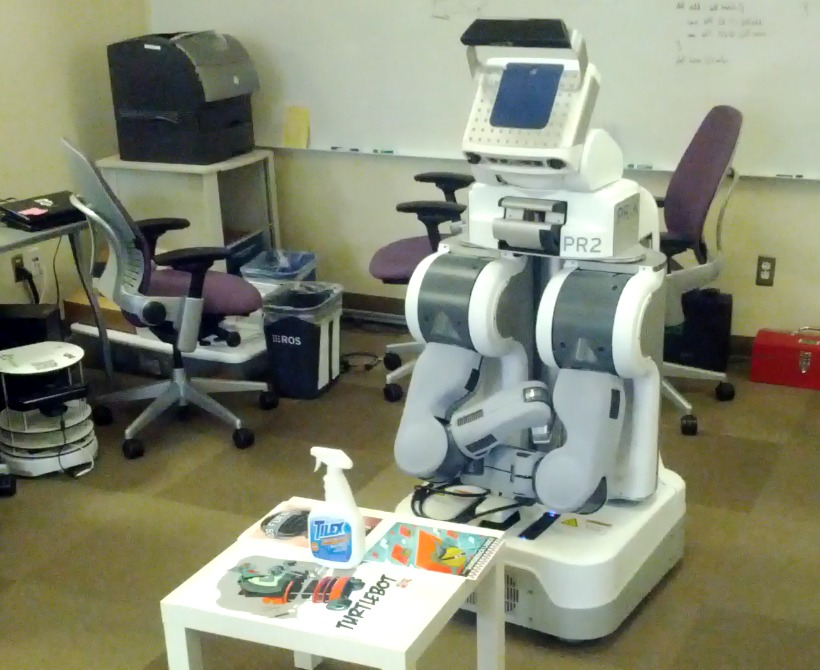
\includegraphics[width=\linewidth]{../tizer/pr2.jpg}
                \caption{PR2 moving around a fixed table}                
        \end{subfigure}%                 
        \end{center}
        
        \begin{subfigure}[b]{0.49\linewidth}
                \centering
                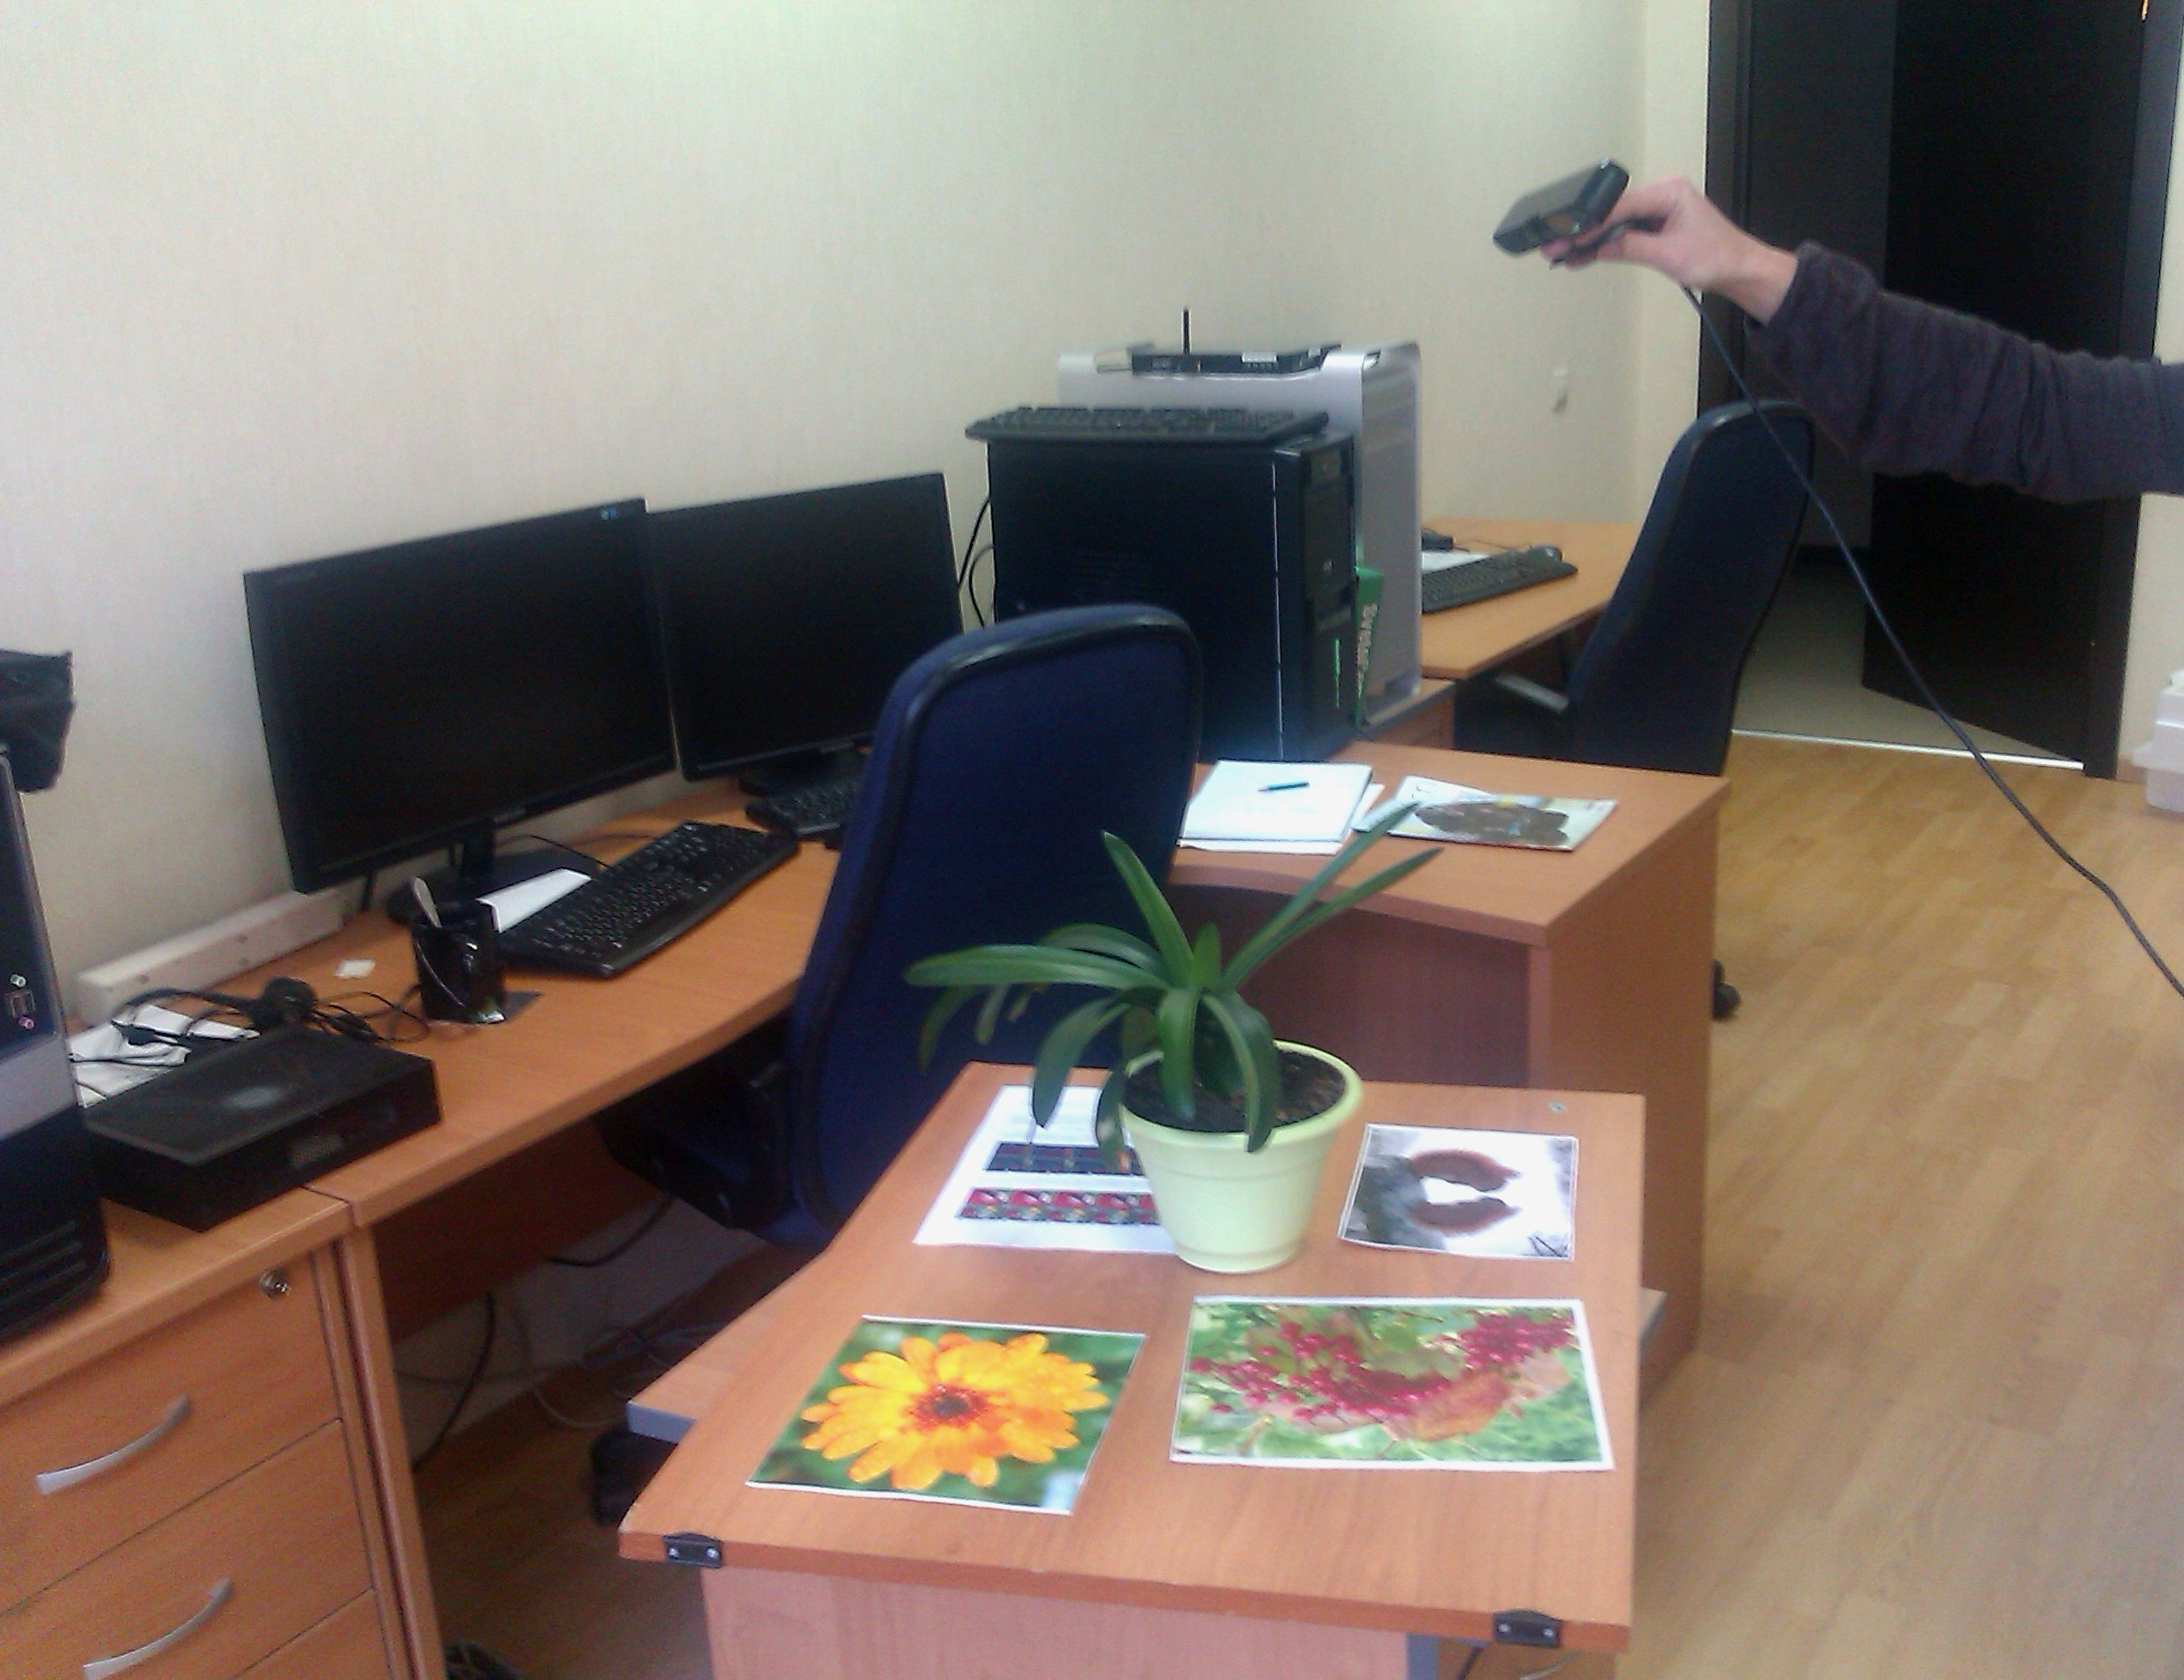
\includegraphics[width=\linewidth]{../tizer/handHeld.jpg}
                \caption{Hand-held sensor moving around a fixed table}
        \end{subfigure}%
        ~ %add desired spacing between images, e. g. ~, \quad, \qquad etc.
          %(or a blank line to force the subfigure onto a new line)
        \begin{subfigure}[b]{0.49\linewidth}
                \centering
                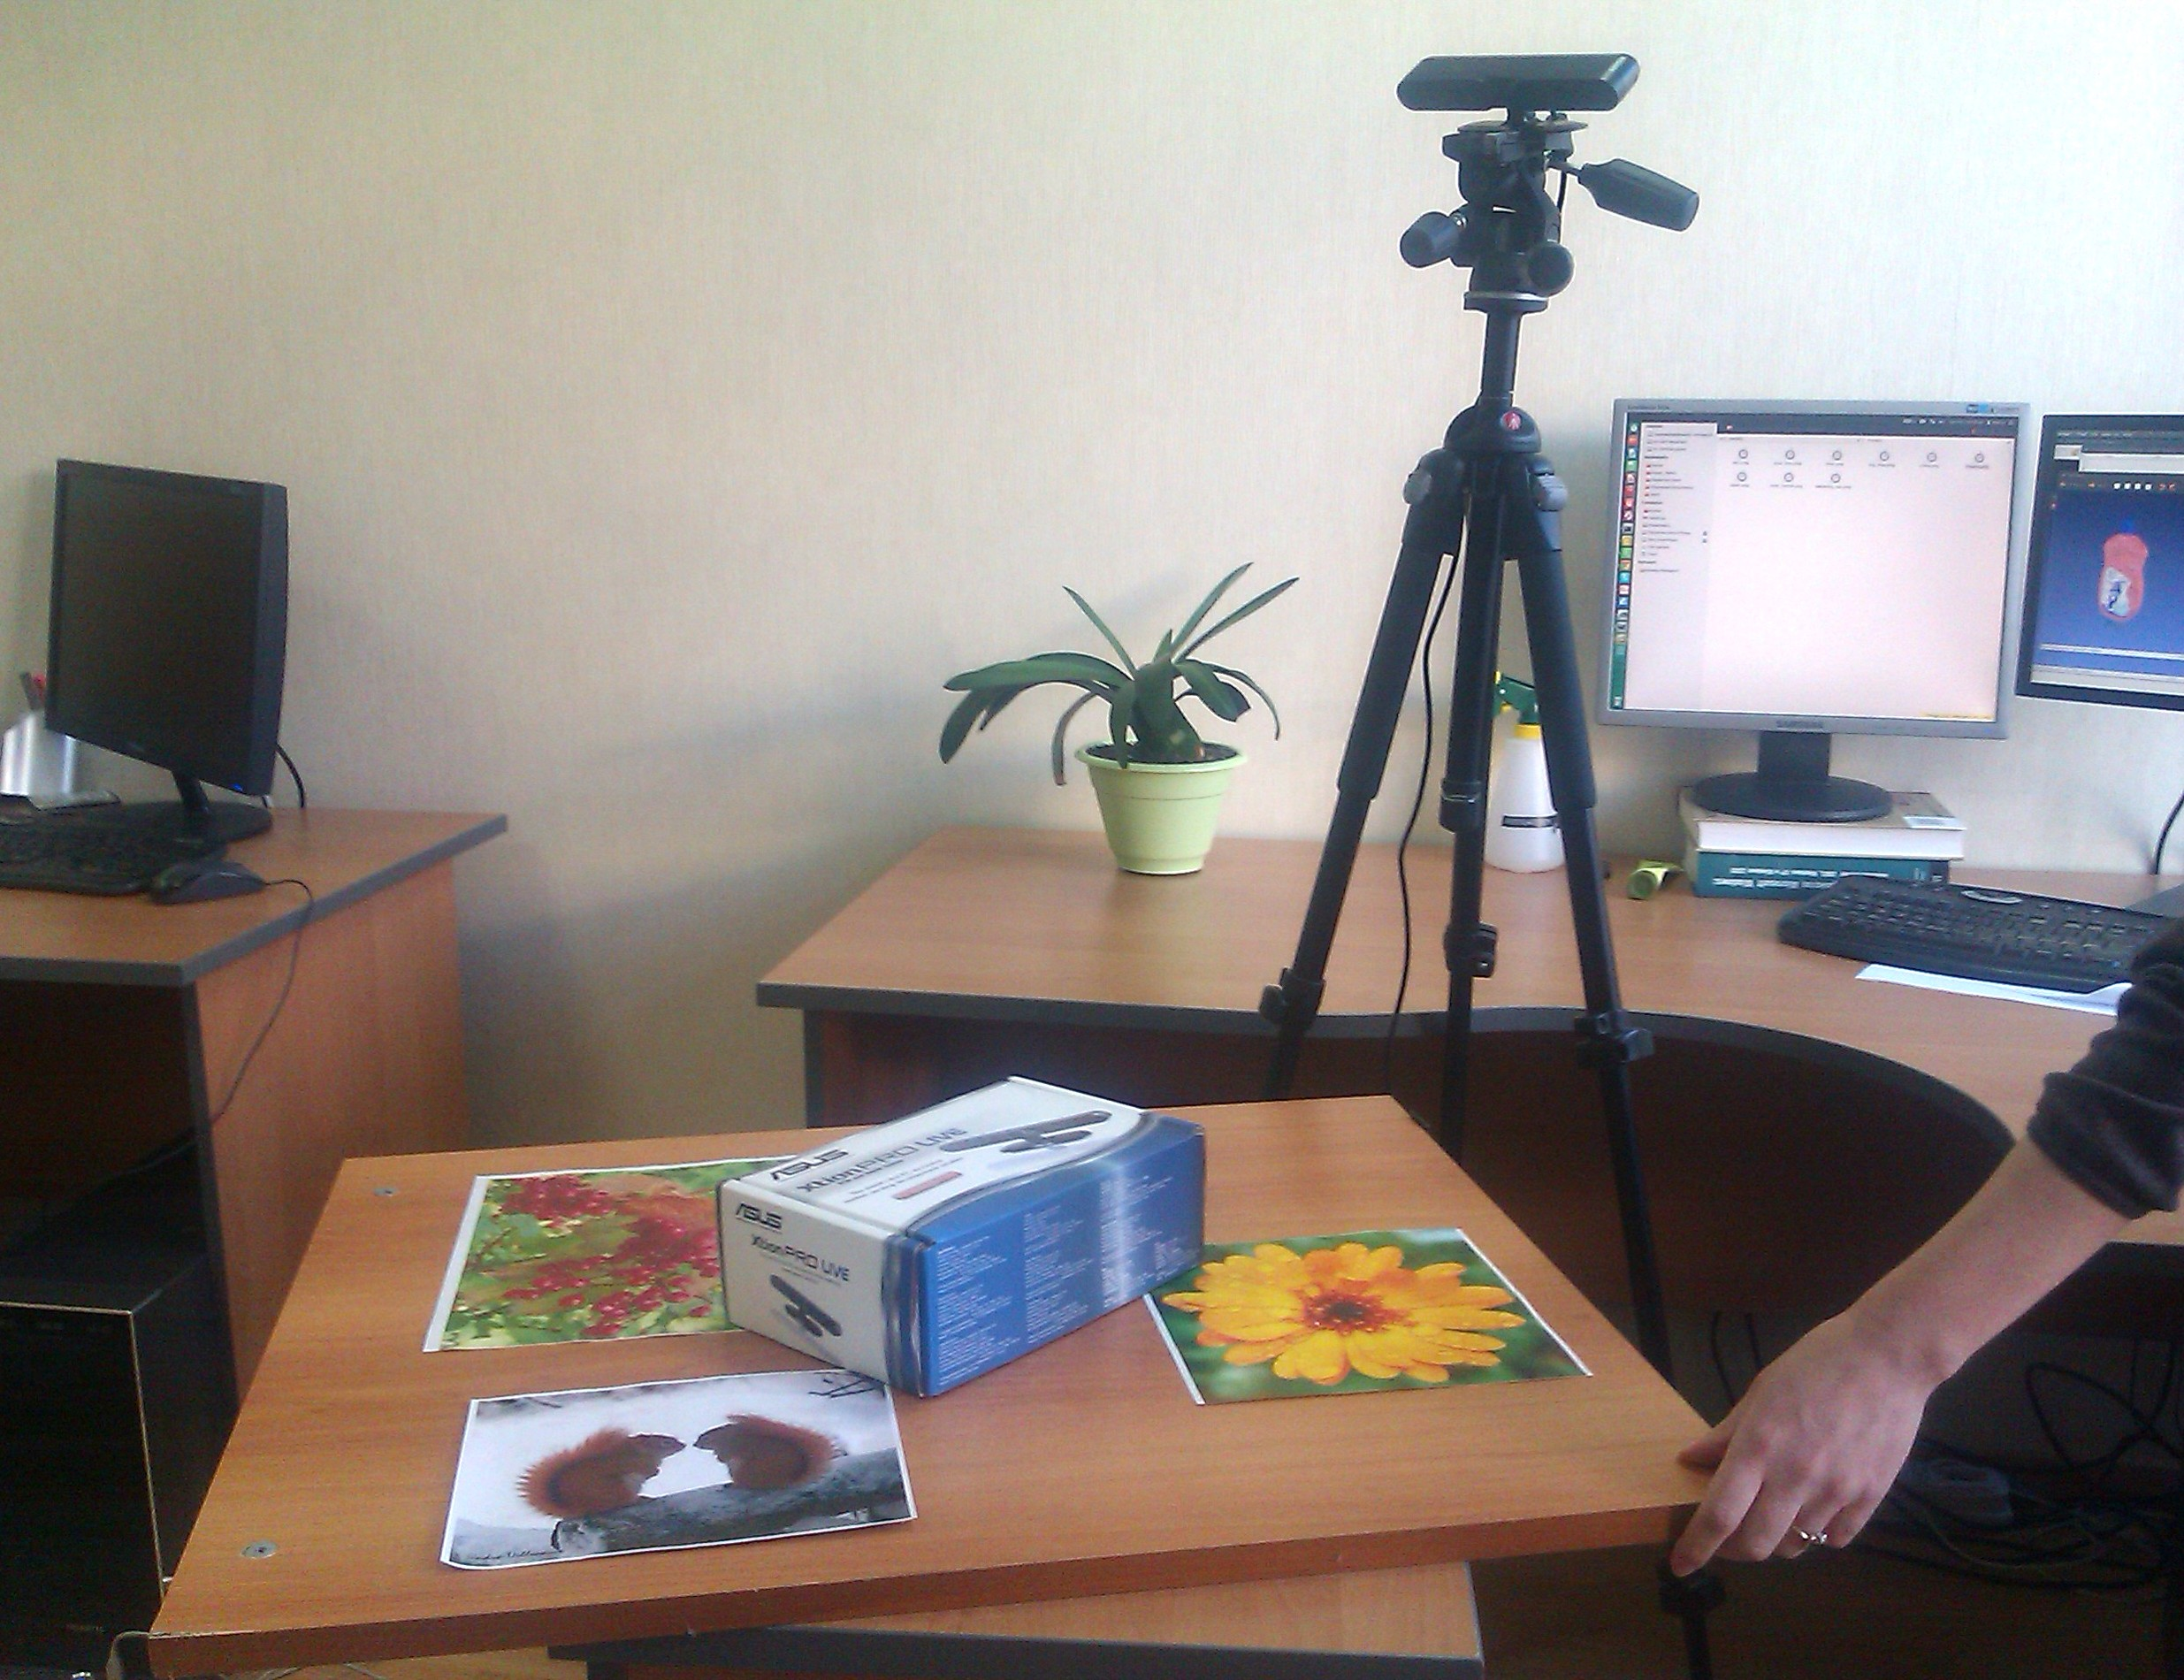
\includegraphics[width=\linewidth]{../tizer/turntable.jpg}
                \caption{Turning table in front of a fixed sensor}
        \end{subfigure}
        
        \begin{subfigure}[b]{\linewidth}
                \centering
                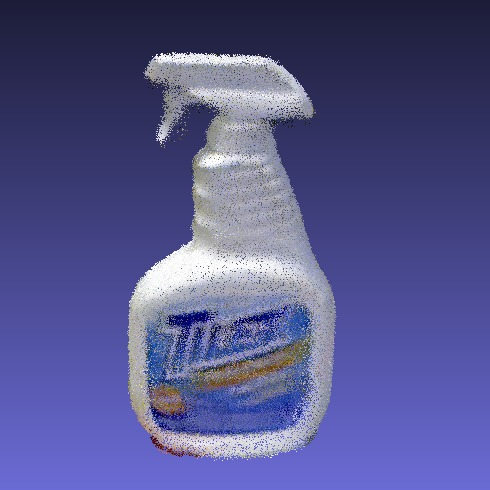
\includegraphics[width=0.49\linewidth]{../tizer/tilexFrontal.jpg}
%                \caption{Segmentation}
%        \end{subfigure}%
%        ~ %add desired spacing between images, e. g. ~, \quad, \qquad etc.
%          %(or a blank line to force the subfigure onto a new line)
%        \begin{subfigure}[b]{0.49\linewidth}
%                \centering
                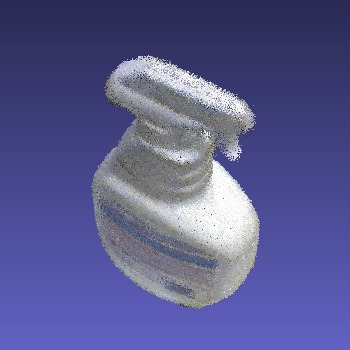
\includegraphics[width=0.49\linewidth]{../tizer/tilexTop.jpg}
                \caption{Model of a "Tilex" bottle captured by a PR2}
        \end{subfigure}
        \caption{Algorithm details: (a)-(c) are the supported 
        capture setups, and (d) shows some results}
        \label{fig:tizer}
\end{figure}


A common object scanning setup is a table or a turntable with
visual markers on it (e.g. chessboards or dot pattern) that
are used for camera pose estimation and sometimes segmentation.
\cite{ectoObjectRecognitionCapture} also 
provides an option to replace special visual markers by arbitrary texture but
there is a training stage in this case:
% replace visual markers after the training? -- it's ambiguous
the user has to capture a canonical image of the empty table from
a planar frontal view before scanning. Preparing the markers
and the training stage for texture is inconvenient for a human and
hard or impossible for a robot. 

Our setup also requires 
texture on a plane but does not track features, hence does not require a training stage.
The table texture is used for the camera motion estimation 
with state-of-the-art dense RGB-D odometry from \cite{steinbrucker2011real}.
We cannot ignore texture because depth-based
techniques for camera motion estimation like ICP \cite{besl1992method} 
are not reliable in our setup with a dominant plane \cite{rusinkiewicz2001efficient}.


For the same reason, we cannot use
the impressive KinectFusion technique \cite{newcombe2011kinectfusion},
which uses ICP for camera poses estimation.
We could intentionally clutter the table but that would bring us back to
an object segmentation problem with possible object occlusions.
Finally, KinectFusion also smoothes captured surfaces too much: \cite{meister2012when} measured that
the system ``can resolve object details with a minimum size of approximately 10mm''.

Another recent approach \cite{stuckler2012model} for 3D model learning 
exploits both RGB and depth information to estimate a camera pose 
in relation to an aggregated scene model represented by the multi-resolution surfels map.
Using RGB data can allow this method to get stable pose estimation
for scenes with a dominant plane. Also this "frame-to-model" camera pose estimation 
(as well as in KinectFusion) leads to less accumulation of the pose estimation error
but small camera pose errors can still exist, which result in
small misalignments of RGB-D scans. Our approach applies global alignment of scans
to increase their consistency to the input RGB and depth data.

Model reconstruction can also be referred to the problem of simultaneous localization
and mapping (SLAM). The SLAM literature is vast, even for approaches using RGB-D
cameras, e.g. \cite{stuckler2012integrating},
\cite{endres2012evaluation}, \cite{henry2012rgb}, \cite{strasdat2011double}. Such approaches are more geared
towards long-lasting navigation and large space mapping while we only focus on relatively small objects.
Also, many of them aim at
real-time runtime on a robot, and they can therefore afford alignment of scans 
as rigid-bodies only. 

The recent work in \cite{ruhnke2012highly} introduced a post-processing procedure for the output of SLAM systems
which considers the registered scans as non-rigid bodies and produces highly accurate
surface of a model by simultaneous refinement of model points positions and camera poses.
Pairwise and global alignment of camera poses and depth maps which include non-rigid 
deformations is also applied in \cite{cui2012algorithms}. Their results include tests on the Kinect
sensor data but their work is mainly focused on Time-of-Flight (ToF) cameras. Considering non-rigid deformations 
of depth maps allowed them to get high quality 3D models even for very noisy ToF depth measurements.
So we also follow the idea of simultaneous optimization of camera poses and model points 
for the final non-rigid refinement. We exploit the knowledge 
about the supported scanning setup and both RGB and depth 
data to produce initial alignment of scans as rigid bodies
and then refine them by such non-rigid optimization.

In this paper, we provide a complete pipeline for object scanning
in the tabletop capturing setup. This setup has natural requirements
with a table and texture for the stable camera pose estimation,
coping with symmetric objects and automatic object segmentation, and it is general enough
to be used by a person or a robot. A base of 42 objects
got successfully scanned from a PR2 robot and a person using a hand-held camera or a Lazy Susan (see 
examples of scanning setups in Fig.~\ref{fig:tizer}).

\section{OVERVIEW OF THE SCANNING PIPELINE}

\label{sec:overview}

We start the overview with a more detailed explanation
of our scanning setup mentioned earlier.

First, we choose a textured table because it solves the following issues:

\begin{itemize}

\item \textit{Automatic object segmentation}. It is easy to find a table plane and segment an object on top of 
it using RGB-D data.
\item \textit{Stable camera pose estimation}. Dense visual odometry methods that are only based on depth measurements,
like ICP, are not reliable in a scene with a prevalent plane \cite{rusinkiewicz2002real}
because planes lack a rich 3D structure (the 2d analogy is matching textureless objects by 
looking for textured 2D 
features). That is why we focus on RGB-D visual odometry instead. Nonetheless, both dense approaches
assume a static scene and can only tolerate slight amounts of noise in movement or environment motion. Therefore,
to obtain a stable camera motion estimation, we run dense odometry with a mask leaving out points that are not on 
the table or object. That also helps us deal with dynamic scenes where there are moving objects e.g. people, pets or 
robots.
\item \textit{Scanning symmetric textureless objects}. Registration of scans for such objects
is most likely to fail if it only uses object points. In order to solve for ambiguities, pose should be known 
beforehand, like in \cite{krainin2011manipulator},
or constraints should be created using some part of a scene with
2D/3D texture. We exploit the plane texture to this end.
\end{itemize}

%TODO: put somewhere?
%We require the full turn
%to get a loop closure in a trajectory which is used to compensate a drift
%of an odometry.

Next, we decide to only make one turn around the table to simplify loop closure detection and pose graph construction as
setting incorrect associations
in the graph can lead to catastrophic implications in the offline graph
optimization \cite{sunderhauf2012switchable}.
However, a complex object like in Figure \ref{fig:pr2} may require a more complicated trajectory
or merging several scanning session together, %TODO: ref
but this is a direction for future work.

Now that the setup is well defined, we can focus on our pipeline. It consists of an online and an 
offline stage. The online part is the capture of RGB-D data,
initial estimation of camera poses using frame-to-frame odometry,
selection of keyframes and detection of loop closure. The offline part performs
global refinement of camera poses and model points given the initial estimate of the online phase.

\section{ONLINE STAGE}

\label{sec:online}

This stage is a real-time set of computations performed during the capture of RGB-D data to initialize 
the offline stage.

We use the dense RGB-D visual odometry
method from \cite{steinbrucker2011real} for the camera motion estimation.
It is accurate and fast enough to apply it online
(execution time of 12.5Hz is reported in \cite{steinbrucker2011real}
on a single Intel Xeon E5520 CPU).
Our open-source implementation\footnote{\label{note1}\href{http://bit.ly/rgbd\_module}{http://bit.ly/rgbd\_module}} of this algorithm
introduces optimization which allows it to work at 23Hz on one core
of Intel Core i5 without using SSE.
It is achieved by only using patches with high gradient in the target intensity image
to compute odometry (the same idea was proposed in \cite{tykkala2011direct} for another odometry algorithm).
Other areas provide less information for alignment
and can be ignored without loss of accuracy; we performed benchmarks 
using the TUM RGB-D datasets \cite{sturm12iros} that corroborated that choice.
% TODO prove it? it's easy to provide results on TUM, but this in not our main goal.  

The RGB-D odometry method assumes absence of motion in a scene which makes it not
% There can exist RGB-D odometry methods that deal with motion.
robust to large movements. To cope with this problem and keep stability, we only run odometry
on the points of the table and the object. The mask of table points
is found in real-time using an approach inspired by \cite{poppinga2008fast}. An object mask is
obtained by extracting points in a virtual 3D prism above the table \cite{rusu2009detecting}.
Using only the points
of a table and an object in the camera pose estimation brings one more advantage:
moving a camera around a fixed table becomes equivalent to rotating
a table in front of a fixed camera. Our system consequently covers the scanning setups both of a hand-held sensor 
and a turntable as we will see in the experiments.

It is still possible to get an incorrect pose from RGB-D odometry
because of light changes or motion blur from hand jitter. We filter out such outliers in the following ways:

\begin{enumerate}
 \item If a returned transformation between two frames is outside the basin of convergence
 of the RGB-D odometry (about 15cm and 15 degrees in our experiments), it is most likely an outlier.
 \item We also warp a source frame using an estimated transformation,
 compute the difference between target and warped frames 
 and filter the transformation out if
 depth and intensity differences are large for many pixels.
\end{enumerate}

%TODO: is there a backward search for a valid transformation?
A pose for each new frame is estimated relatively to the last frame
with a valid transformation from the odometry.

The frame-to-frame estimation of camera poses from the RGB-D 
odometry results in a drift. It is usually not too large in our case
due to high accuracy of the used odometry method \cite{steinbrucker2011real}
and only one loop around the object.
Still, it should be compensated and we use loop closure to this end.
%TODO: how much is "large enough"?
When the length of the trajectory is large enough, we begin to estimate the
odometry transformation between each current frame and the starting one. 
If the returned transformation passes through the described filters, 
it means the current pose is close to the first one and 
the trajectory has been closed. When the loop closure is detected 
the capture is stopped.

Finally, during capture, we keep track of key frames by analyzing the translation and rotation differences between a 
current frame and the last keyframe.

To summarize, each frame is passed through the steps:

\begin{enumerate}
 \item plane and object segmentation,
 \item odometry estimation and outliers filtering,
 \item the check: is it a keyframe?
 \item the check: is it loop closure?
\end{enumerate}

We also should note that loop closure detection using the RGB-D odometry requires
the last pose of a camera to be in a basin of
the algorithm convergence (about 15cm and 15 degrees as we mentioned earlier) from the first pose. 
To allow a larger difference between the first and the last frames
another approach could be used in detection of loop closure. We tried to use visual descriptors, like
SIFT \cite{lowe2004distinctive}, SURF \cite{bay2006surf}, ORB \cite{rublee2011orb}, but they failed to match even
relatively close frames due to large affine distortions.
ASIFT \cite{morel2009asift} was able to overcome this problem
and perfectly coped with the task in our experiments;
it however has to be strongly optimized before it can be used in an online application.

The output of the online part is a set of consecutive keyframes with 
estimated poses and the transformation between the first and the last 
keyframes from loop closure.


\section{OFFLINE STAGE}

\label{sec:offline}

The purpose of the offline processing is to refine the online-estimated 
camera poses and object points to get a model maximally 
consistent with the captured RGB-D data. We achieve this in three steps by 
solving least squares optimization problems. The cost function is extended at each step 
by introducing additional terms which can be reliably computed
thanks to refinement from the previous stage.

%TODO is it clear that constrains are the same but they are with new data (new corresps, etc.)?

\subsection{First Step}

The input of the offline stage is a set of initial camera poses $\{x_n^{(0)},~n=1,\dots, N\}$ 
estimated by accumulating consecutive frame-to-frame odometry transformations 
$\{z_n,~n=1,\dots, N-1\}$  
(where $z_n$ is the odometry transformation from the frame $n+1$ to the frame $n$)
%from each 
%current frame to the previous one
and the loop closure constraint $z_{N}$, 
i.e. odometry transformation from the last frame to the first one.

\begin{figure}[t]
	\centering
        \begin{subfigure}[b]{0.45\linewidth}
                \centering
                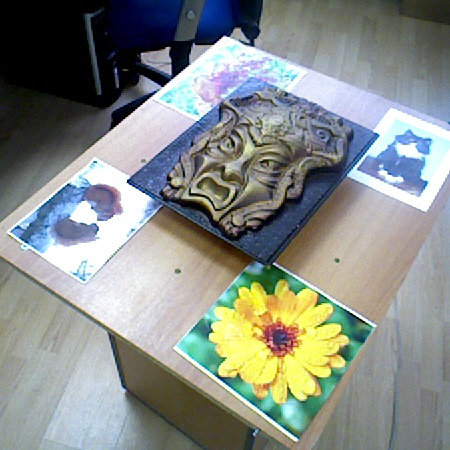
\includegraphics[width=\linewidth]{../models/gorgon_train.jpg}
                \caption{}
        \end{subfigure}%
        ~ %add desired spacing between images, e. g. ~, \quad, \qquad etc.
          %(or a blank line to force the subfigure onto a new line)
        \begin{subfigure}[b]{0.45\linewidth}
                \centering
                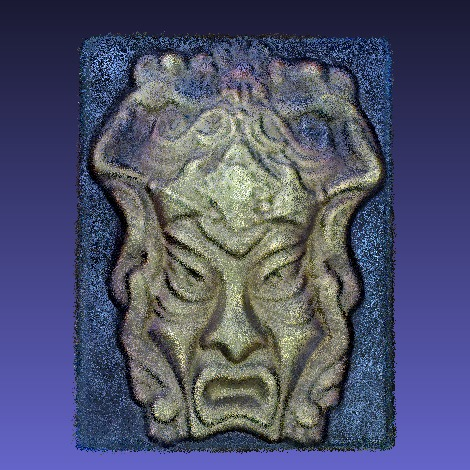
\includegraphics[width=\linewidth]{../models/gorgon_color_model.jpg}
                \caption{}
        \end{subfigure}

        \centering
        \begin{subfigure}[b]{0.45\linewidth}
                \centering
                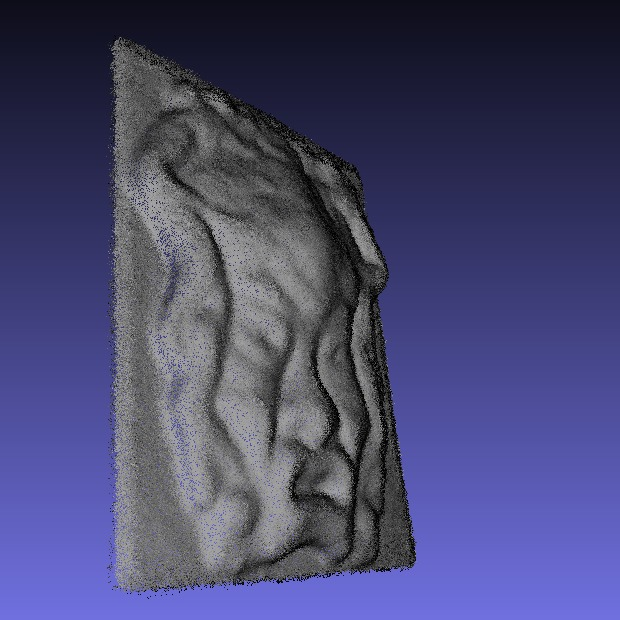
\includegraphics[width=\linewidth]{../models/gorgon_gray_model1.jpg}
                \caption{}
        \end{subfigure}%
        ~ %add desired spacing between images, e. g. ~, \quad, \qquad etc.
          %(or a blank line to force the subfigure onto a new line)
        \begin{subfigure}[b]{0.45\linewidth}
                \centering
                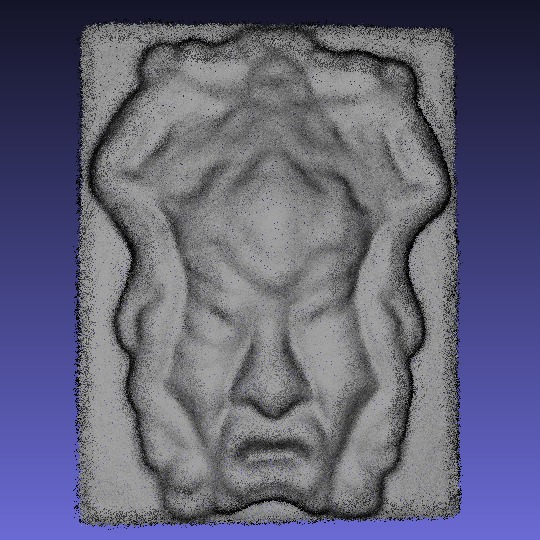
\includegraphics[width=\linewidth]{../models/gorgon_gray_model.jpg}
                \caption{}
        \end{subfigure}
        \caption{Scanning the relief picture of Gorgon: (a) train image example,
        (b) colored model (point cloud), (c,d) uncolored point cloud}
        \label{fig:gorgon}
\end{figure}

First, we compensate the drift in frame-to-frame estimated camera poses and 
make them consistent to the odometry constraints (including the transformation from the last pose
to the first one) by minimizing the following cost function
with regard to camera poses $x_{1:N}$:
\begin{equation} \label{eq:ffirst}
F_{SE3}(x_{1:N}) = \sum_n (z_n \ominus y_n)^T \Omega_{SE3} (z_n \ominus y_n),
\end{equation}
where $\ominus$ is the inverse compounding operator \cite{lu1997globally},
%TODO give definition of the operator in text?
$y_n=x_{n+1} \ominus x_{n}$ ($n=1,\dots, N-1$), $y_N=x_N \ominus x_1$,
the matrix $\Omega_{SE3}$ is an information matrix that weighs an odometry uncertainty \cite{kuemmerle2011g2o}.
%TODO say that it's diagonal matrix here?

\subsection{Second Step}

The first step does not use RGB-D information directly which results in
slightly misaligned frames. Therefore, to achieve better consistency among all RGB-D scans, we add an RGB-D term to 
refine the camera poses in a second step.
As the first step improved pose accuracy by exploiting loop closure, 
corresponding points between two frames can now be found using
the fast projective data association algorithm \cite{rusinkiewicz2001efficient}.
For each pair of corresponding 3D points from each pair of frames, two minimization terms are added: one 
for their 3D distance and one for their image intensity difference.

The cost function responsible for the shape 
consistency is the sum of the ICP odometry terms:
\begin{equation} \label{eq:ficp}
    F_{ICP}(x_{1:N}) = \sum_{n,m,i,j} \Delta p_{nmij}^T \Omega_{mj} \Delta p_{nmij},
\end{equation}
\begin{equation}
    \Delta p_{nmij}=(p_{ni} \oplus x_n) \ominus x_m - p_{mj},
\end{equation}
where the summation is done over all corresponding points, $p_{nk}$ is the $k^{th}$ 3D point of 
the $n^{th}$ frame, $\oplus$ is 
the compounding operator \cite{lu1997globally} and $\Omega_{mj}$ is 
the information matrix that results in the point-to-plane 
distances in \eqref{eq:ficp}.
%TODO clarify this?

\begin{figure}[t]
	\centering
        \begin{subfigure}[b]{0.45\linewidth}
                \centering
                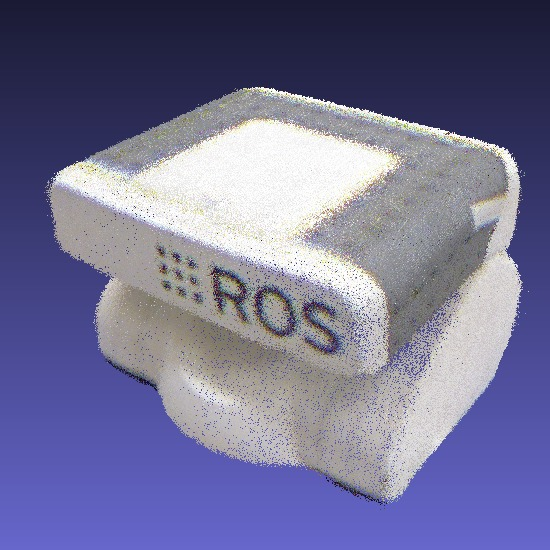
\includegraphics[width=\linewidth]{../models/pr2_full.jpg}
                \caption{}
        \end{subfigure}%
        ~ %add desired spacing between images, e. g. ~, \quad, \qquad etc.
          %(or a blank line to force the subfigure onto a new line)
        \begin{subfigure}[b]{0.45\linewidth}
                \centering
                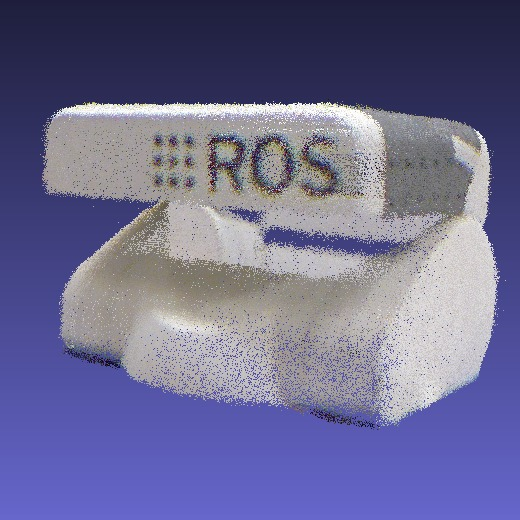
\includegraphics[width=\linewidth]{../models/pr2_holes.jpg}
                \caption{}
        \end{subfigure}
        \caption{Example of a hole problem due to self-occlusions:
        (a) final PR2 head model as seen from one of the capture views,
        (b) newly generated viewpoint that is lower than the original camera trajectory: a hole under 
        the top part of the head is visible}
        \label{fig:pr2}
\end{figure}

The cost function responsible for the intensity consistency is
the sum of the RGB-D odometry terms:
\begin{multline} \label{eq:frgbd}
F_{RGBD}(x_{1:N}) = \\
= \omega_{rgbd} \sum_{n,m,i} \biggl[I_n(\pi p_{ni}) - I_m\Bigl(\pi \bigl((p_{ni} \oplus x_n) \ominus x_m\bigr)\Bigr) \biggr]^2,
\end{multline}
where $I_n$ is the intensity image of the $n$-th frame, $\pi$ is an image projection function, $\omega_{rgbd}$
is a weight of the RGB-D term.

To summarize, the following function is minimized during the second step:
\begin{equation} \label{eq:fsecond}
F_{SE3}(x_{1:N}) + F_{ICP}(x_{1:N}) + F_{RGBD}(x_{1:N}).
\end{equation}

In order to increase the basin of convergence,
we minimize \eqref{eq:fsecond} using a coarse-to-fine approach.
% It is not the defininition of our coarse-to-fine approach, it is just a remark
The correspondences between frames are recomputed
after each iteration of each pyramid level.

The optimization of the function \eqref{eq:fsecond} is run 
twice for different points. The first time, the points of the table and object are used because 
the textured table points give necessary constraints in the case of symmetric and textureless object.
The second time, \eqref{eq:fsecond} is minimized using only object points to refine 
camera poses relatively to the interesting parts of the scans only.

\subsection{Third Step}

The second optimization step gives accurate camera poses and properly aligned scans
as rigid bodies but the depth measurement noise leads to some misalignment. The third step produces a 
final accurate model by
simultaneously optimizing object points coordinates and camera poses.

This step exploits the idea of \cite{ruhnke2012highly} but our version 
is simplified due to the previous steps: 

\begin{itemize}
 \item As we already have well-aligned scans at this stage, we can apply 
 the fast projective algorithm \cite{rusinkiewicz2001efficient} 
 (with filtering by differences in depth values, 
 normals and intensity) to find correspondences instead of the slower
% Ruhnke didn't propse this method, he just uses it
 normal-shooting method that \cite{ruhnke2012highly} uses.
 %TODO add a direct link to the normal-shooting?
 \item We consider each object 3D point of each frame as 
 a surfel because we don't aim at large space model refinement as in \cite{ruhnke2012highly}:
 it is not necessary for us to use a more compact scan surface representation by covering several pixels 
 by one surfel.
 \item After the surfel 3D position is refined, we only update the depth value 
 of a pixel in the original pixel depth map. This conforms with the purpose of
 refining noisy depth measurements using information from other scans.
\end{itemize}

With these remarks the error function for the surfel positions refinement 
$F_{model}(x_{1:N}, M)$ (where $M$ is a set of 3D points from 
all frames) in our approach is the same as formula (11) in \cite{ruhnke2012highly}.

To summarize the third step, we minimize the following function:
\begin{multline} \label{eq:fthird}
F_{SE3}(x_{1:N}) + F_{ICP}(x_{1:N}) + F_{RGBD}(x_{1:N}) + \\
+ F_{model}(x_{1:N}, M).
\end{multline}

After \eqref{eq:fthird} is minimized we filter out the points 
that have no or few (less than 3) correspondences in
all other frames because they were not refined or the refinement result
is unreliable due to a small number of used correspondences.

In order to solve the least squares optimization problems 
of the three steps \eqref{eq:ffirst}, \eqref{eq:fsecond} and \eqref{eq:fthird} 
we formulate them as graph-based optimization tasks.
These tasks are solved by applying the g2o framework 
\cite{kuemmerle2011g2o} which exploits sparseness of the graph structure.

The output of the offline stage is the final model representing
a colored point cloud where the color of each 3D point is taken 
by its pixel coordinates from the frame where the point was originaly 
captured (see an example in Fig.~\ref{fig:gorgon}).

\begin{figure}[th]
        %\begin{center}
	\centering
        \begin{subfigure}[b]{0.5\linewidth}
                \centering
                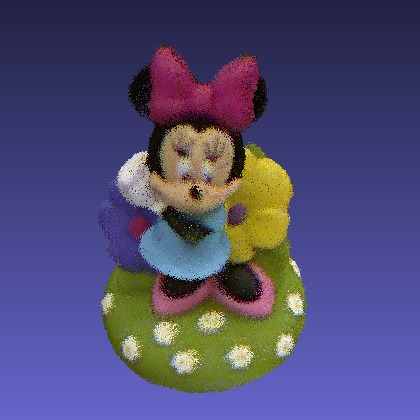
\includegraphics[width=\linewidth]{../models/mouse.jpg}
                %\caption{PR2 moving around a fixed table}                
        \end{subfigure}%                 
        %\end{center}
        \begin{subfigure}[b]{0.5\linewidth}
                \centering
                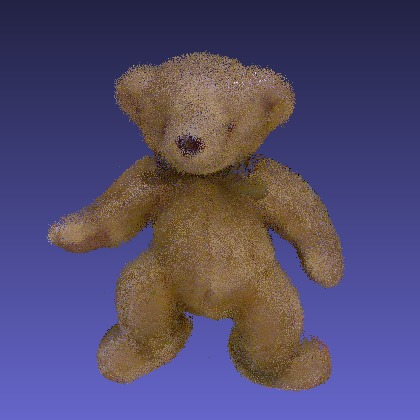
\includegraphics[width=\linewidth]{../models/bear.jpg}
                %\caption{Hand-held sensor moving around a fixed table}
        \end{subfigure}
        
        
        \begin{subfigure}[b]{0.5\linewidth}
                \centering
                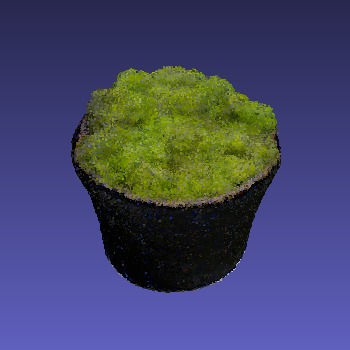
\includegraphics[width=\linewidth]{../models/plant.jpg}
                %\caption{Turned table beyond a fixed sensor}
        \end{subfigure}%
        \begin{subfigure}[b]{0.5\linewidth}
                \centering
                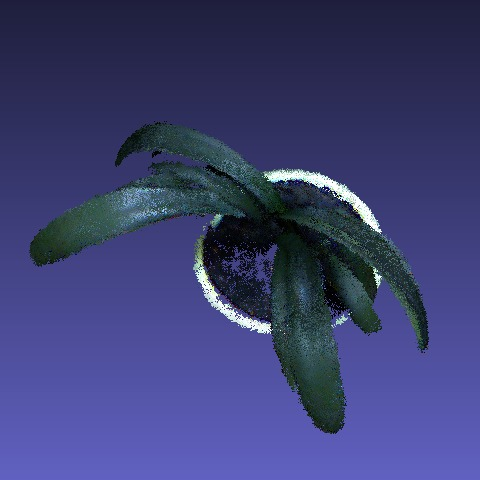
\includegraphics[width=\linewidth]{../models/clivia.jpg}
                %\caption{Turned table beyond a fixed sensor}
        \end{subfigure}
        
        \begin{subfigure}[b]{0.333333\linewidth}
                \centering
                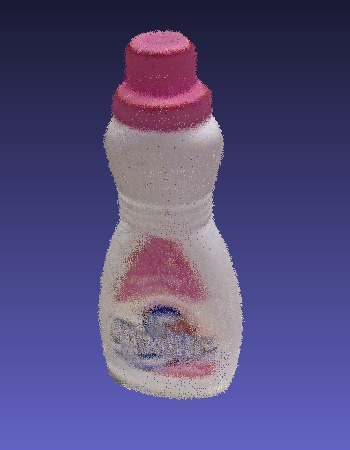
\includegraphics[width=\linewidth]{../models/rose_bottle.jpg}
                %\caption{Turned table beyond a fixed sensor}
        \end{subfigure}%
        \begin{subfigure}[b]{0.333333\linewidth}
                \centering
                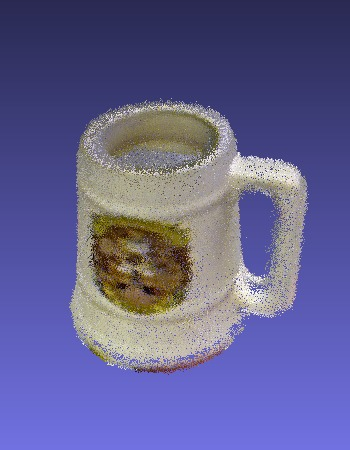
\includegraphics[width=\linewidth]{../models/big_mug.jpg}
                %\caption{Turned table beyond a fixed sensor}
        \end{subfigure}%
        \begin{subfigure}[b]{0.3333\linewidth}
                \centering
                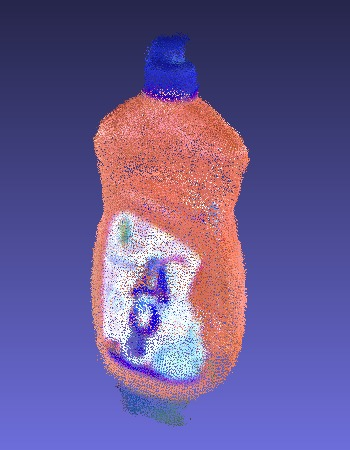
\includegraphics[width=\linewidth]{../models/aos.jpg}
                %\caption{Turned table beyond a fixed sensor}
        \end{subfigure}
        
        \begin{subfigure}[b]{0.5\linewidth}
                \centering
                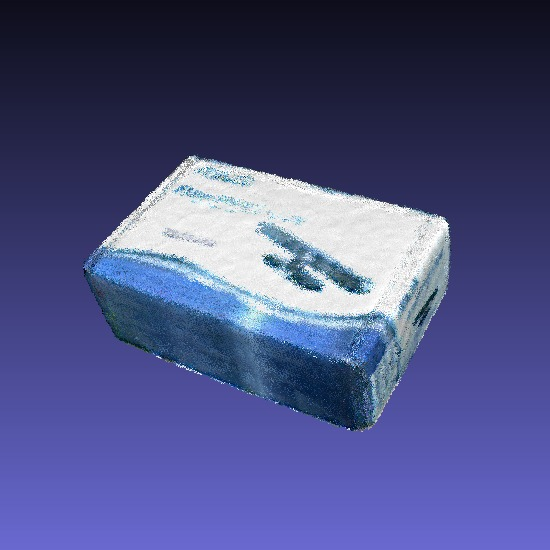
\includegraphics[width=\linewidth]{../models/asus_box.jpg}
                %\caption{Turned table beyond a fixed sensor}
        \end{subfigure}%
        \begin{subfigure}[b]{0.5\linewidth}
                \centering
                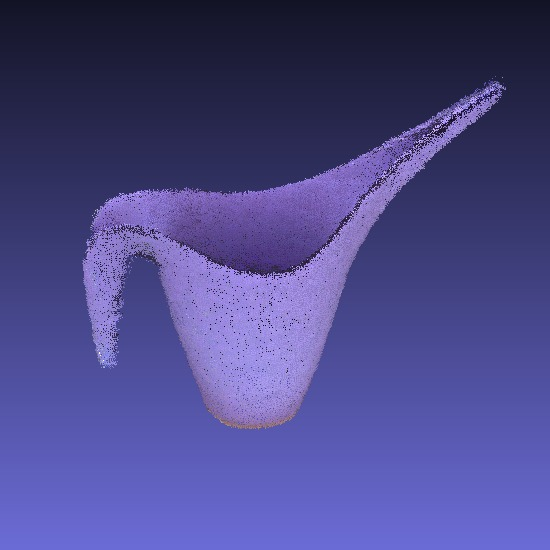
\includegraphics[width=\linewidth]{../models/watering_can.jpg}
                %\caption{Turned table beyond a fixed sensor}
        \end{subfigure}
        \caption{Examples of reconstructed models}
        \label{fig:results}
\end{figure}

\section{RESULTS}

\label{sec:experiments}

The presented system was tested on three capturing scenarios:

\begin{itemize}
 \item A person with a hand-held camera and an object placed on a fixed table.
 \item A PR2 robot with its RGB-D sensor looking at an object on a fixed table and rotating around it.
 \item A fixed camera and an object on a Lazy Susan.
\end{itemize}

% This formulation stresses that all objects were scanned successfully
The algorithm successfully produced accurate models 
on a dataset of 42 household objects. We show several examples in Fig.~\ref{fig:results}.

The offline refinement of camera poses 
and model points takes about 5-10 minutes for one model on an Intel Core i5 using up to 12 Gb of RAM
depending on object size.

We also experimented building meshes from those point clouds using 
the ball pivoting algorithm \cite{bernardini1999ball}
implemented in MeshLab \cite{meshlab}. The accuracy of 
the point cloud allows building high quality meshes but the results do have some problems. One of the important issues 
is holes in 
the mesh due to absent measurements of an RGB-D camera in occluded parts of the object surface 
(see the Fig.~\ref{fig:pr2} for an illustration of the problem).
Allowing an arbitrary camera 
trajectory would reduce unobserved object area and give more complete
point clouds and meshes. Another potential direction for future work is texture projection on the mesh.


\section{CONCLUSION}

This paper presents a tabletop object scanning pipeline which, in addition to producing accurate 3D models from RGB-D 
data, also offers an easy-to-use set up. The plane and single loop closure are the only requirements and the online 
processing computation helps cleaning the data and providing feedback during the capture.
It is convenient enough for usage by a person and also makes a robot closer
to autonomous acquisition of a 3D model as was shown during the capture of our dataset.

Future work includes meshing of the object as well as multiple loop handling for complex objects.

The code of the system is available as open-source at
\href{http://bit.ly/reconst3d}{http://bit.ly/reconst3d}.

\addtolength{\textheight}{-8.1cm}   % This command serves to balance the column lengths
                                  % on the last page of the document manually. It shortens
                                  % the textheight of the last page by a suitable amount.
                                  % This command does not take effect until the next page
                                  % so it should come on the page before the last. Make
                                  % sure that you do not shorten the textheight too much.

%%%%%%%%%%%%%%%%%%%%%%%%%%%%%%%%%%%%%%%%%%%%%%%%%%%%%%%%%%%%%%%%%%%%%%%%%%%%%%%%

\bibliographystyle{ieeetr}
\bibliography{../references.bib}




\end{document}
